\section{Configuration Table}\label{sec:first-configuration-table}
This section will describe what a configuration table is, and how our configuration table looks for the first sprint.

A configuration table, is a table, with information about the project status. 
The table will help get a better overview of the solution being made, and why the problem needs to be solved.
A benefit of the configuration table, is that at all times it is visible what the given sprint focus is, and when review of the solution and other things is needed, the configuration table has columns with criteria for the solution.

\begin{figure}[h]
    \centering
    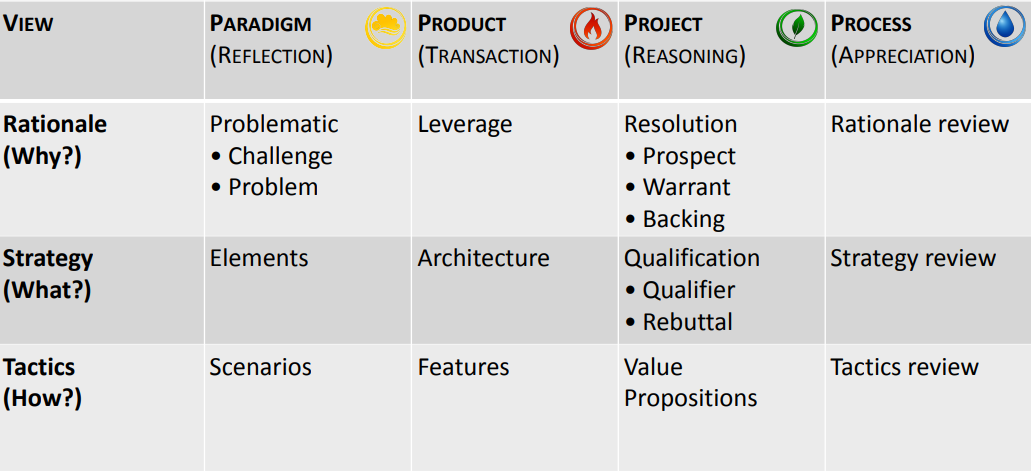
\includegraphics[width=\linewidth]{images/configurationTableExample.png}
    \caption{Structure of a Configuration table.}
    \label{fig:example-configuration-table}
\end{figure}

~\autoref{fig:example-configuration-table} shows the stucture of a configuration table.
The confiugration table has three layers, \textbf{Rationale}, \textbf{Tactics} and \textbf{Strategy}, and are organised into four "views".
Each of these layer has its own area of view in the given project.
Some of these share some categories with one another.
The confiugration table is organised into four "views", which are:

\begin{itemize}
    \item Paradigm - Used as the understanding of the problem
    \item Product - Used to describe how the constructive parts of the solution could be designed
    \item Project - Used to reason about the purpose and our overall idea in the project.
    \item Process - Used to determine if we are on the right track or not, in solving the problem. 
\end{itemize}

The rationale layer is known as the "why" layer.
Why are we trying to solve the problem we have, and which leverage points is used to solve the problem.
Under Problematic, there are \textbf{Challenge} and \textbf{Problem}, also known in the first iteration, as the initial problem.
Next is the \textbf{Leverage}, which is the leverage points that where found in the pre-project.
Next, the resolution, which is the prospect, warrant, and backing. 
Here we look at the \textbf{Prospect}, which is the solution.
The \textbf{Warrant} is a statement about why it is important to solve the problem at hand, and the \textbf{Backing} is why we think that the prospect is a useful solution to the problem.
The last cell is the rationale review, which looks at the \textbf{Criteria for our resolution}.
This cell is meant to be a checklist, that can be reviewed, for example at the end of a sprint.
The rationale layer also involves architecture, which will be described in the strategy layer paragraph.

The strategy is the "what" layer.
This layer concerns the organization of our actions and how to model our platform.
First is the \textbf{Elements}, which are core objects or events in our problem domain.
The \textbf{Architecture} is the conceptual structure and logical organization, of our software system.
Next is the \textbf{Qualification}, which is the \textbf{Qualifier} and \textbf{Rebuttal}.
The qualifier states the limitations of our solution.
The rebuttal is then a statement about why this is okay or good enough.
The last thing in this layer is the \textbf{Strategy review}, where we state the \textbf{Criteria for Architecture}.
Just as in the Rationale review cell, there should be made a checklist of questions that can be reviwed, about the architecture.
One of these could be if the architecture is feasible or not.
The strategy layer also involves leverage and features.

The Tactics layer is the "how" layer.
How do we benefit from our solution, and which features do is needed in order to get value out of it.
The first cell is the \textbf{Scenarios}, which is statements about which scenarios, this prospect should focus on.
Next, is the \textbf{Features}, which are attributes in our software, which will provide value propositions.
Then \textbf{Value Propostions}, which is something that is desired as a (partial) solution to our problem.
Lastly we state the \textbf{Criteria for Value Propostions}.
Do we get enough value out of our solution, or not.
The Tactics layer also concerns about the elements and architecture.

All of this leads us to our first configuration table, which can be seen in~\autoref{tab:first-configuration-table}

\begin{landscape}
    \begin{table}[]
        \tiny
    \begin{tabular}{|l|l|l|l|l|}
    \hline
    View & \multicolumn{1}{c|} {Paradigm} & \multicolumn{1}{c|} {Product} & \multicolumn{1}{c|}{Project} & Process \\ \hline
    Value & \multicolumn{1}{c|}{Reflection} & \multicolumn{1}{c|}{Transaction} & \multicolumn{1}{c|}{Reasoning} & Appreciation \\ \hline
    Rationale & \begin{tabular}[c]{@{}l@{}}Problematic:\\ \\ Challenge: Improve the communication \\ between customers and developers in \\ an Agile Software Development Process.\\ \\ Problem: The communication between \\ customers and developers are one of the \\ most challenging aspects of the \\ development process.\end{tabular} & \begin{tabular}[c]{@{}l@{}}Leverage:\\
        \begin{minipage} [t] {0.3\textwidth} 
            \begin{itemize}
            \item Docker
            \item Flutter
            \item DotNet
            \item Entity Framework
            \item PostgreSQL
            \item JavaScript Frameworks
           \end{itemize} 
          \end{minipage} 
    \end{tabular} & \begin{tabular}[c]{@{}l@{}}Resolution:\\ \\ Prospect: The communication \\ between developers and \\ product owners will become easy.\\ \\ Warrant: Because software \\ development is expensive, \\ and could reduce the \\ cost and increase the quality\\ \\ Backing: Inexpensive, \\ popular platform. Extensible\end{tabular} 
            & \begin{tabular}[c]{@{}l@{}}Criteria for resolution expectations:\\ 
                \begin{minipage} [t] {0.3\textwidth} 
                    \begin{itemize}
                    \item Is the problem still worth solving
                    \item Does the proposed solution solve the problem
                    \item Have we used the correct leverage points
                   \end{itemize} 
                  \end{minipage}    
                \\ \\ Findings:\end{tabular} \\ \hline
    Strategy  & \begin{tabular}[c]{@{}l@{}}Elements \& Ecology:\\ 
        \begin{minipage} [t] {0.35\textwidth} 
            \begin{itemize}
            \item The product owners problem domain will be visible
            \item The product owner will have more direct communication with the developers
            \item Making the development process transparent
           \end{itemize} 
          \end{minipage} 
    \end{tabular} & \begin{tabular}[c]{@{}l@{}}Architecture:\\ 
        \begin{minipage} [t] {0.2\textwidth} 
            \begin{itemize}
            \item Digital app editor module
            \item Digital issue tracking module
            \item Digital communication module
           \end{itemize} 
          \end{minipage}\end{tabular} & \begin{tabular}[c]{@{}l@{}}Qualification:\\ \\ Qualifier: Requires some \\ knowledge about using apps\\ \\ Rebuttal: Most people \\ have this skill\end{tabular} 
            & \begin{tabular}[c]{@{}l@{}}Criteria for architecture expectations: \\
            \begin{minipage} [t] {0.3\textwidth} 
                \begin{itemize}
                \item Is the architecture feasible
                \item Is the product user-friendly
               \end{itemize} 
              \end{minipage} \\
\\ Findings:\end{tabular} \\ \hline
    Tactics   & \begin{tabular}[c]{@{}l@{}}Scenarios:\\ 
        \begin{minipage} [t] {0.3\textwidth} 
            \begin{itemize}
            \item Product owner used the system to create tasks for developers
            \item Developers can take tasks and solve them
            \item The Product owner can at any time see how a task is going and see the progress
           \end{itemize} 
          \end{minipage} 
         \end{tabular} & \begin{tabular}[c]{@{}l@{}}Features:\\ 
            \begin{minipage} [t] {0.3\textwidth} 
                \begin{itemize}
                \item App editor where the Product owner can make their requirements visible
                \item Translate App editor to developer requirements
                \item The Product owner can at any time see how a task is going and see the progress
               \end{itemize} 
              \end{minipage} 
    \end{tabular} & \begin{tabular}[c]{@{}l@{}}Value Propostions:\\
        \begin{minipage} [t] {0.3\textwidth} 
            \begin{itemize}
            \item Translate customer requirements to product requirements
           \end{itemize} 
          \end{minipage} 
         \end{tabular} & 
    \begin{tabular}[c]{@{}l@{}}Criteria for value propostions \\ expectations: \\
        \begin{minipage} [t] {0.3\textwidth} 
            \begin{itemize}
            \item Is the translation effective
           \end{itemize} 
          \end{minipage} 
         \\ \\ Findings:\end{tabular} \\ \hline
    \end{tabular}
    \caption{First configuration table, named Anne.}
    \label{tab:first-configuration-table}
    \end{table}
\end{landscape}
